
%----------------------------------------------------------------------------
\chapter{Overview of the approach}
%----------------------------------------------------------------------------

%%
%% Futásidejű dolgok és kódgenerálás is!
%%


\begin{figure}[h]
	\begin{center}
		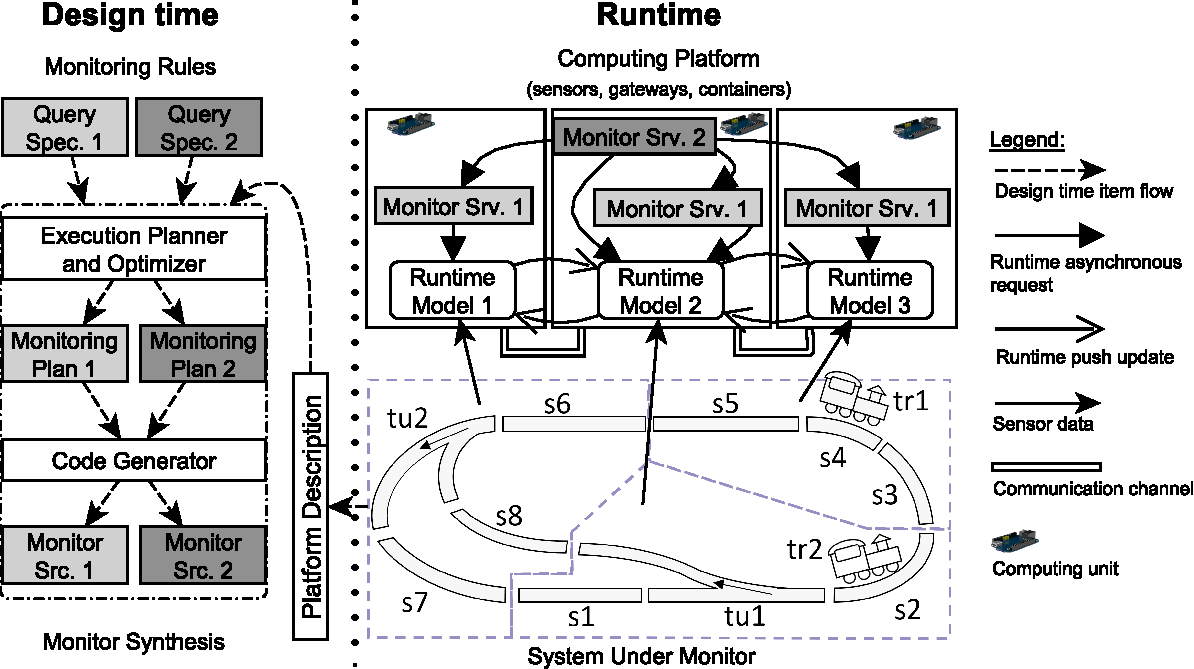
\includegraphics[width=\textwidth]{figures/fase-overview-crop.pdf}
	\end{center}
\end{figure}




\section{Overview of the query compilation workflow}

\begin{figure}[h]
	\begin{center}
		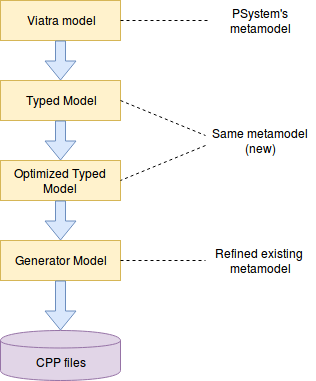
\includegraphics[width=0.5\textwidth]{figures/workflow.png}
	\end{center}
\end{figure}



\section{Distributed runtime model}

\begin{figure}[h]
	\begin{center}
		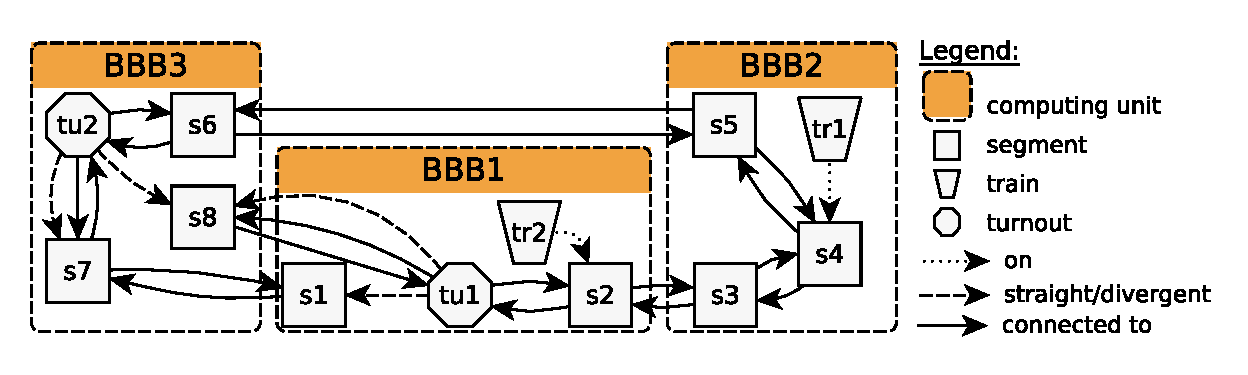
\includegraphics[width=0.9\textwidth]{figures/runtime-snapshot.pdf}
	\end{center}
\end{figure}


\section{Distributed query execution}


\subsection{Distributed local search}

As models are stored on different computational units we still needs to find matches, that can span over multiple model parts. To find matches for a pattern local search algorithm is used in a distributed way. Search operations are being executed locally, and if the next operation needs to be executed on multiple nodes, the search context, (ie.\ the bound variables and the operations number) are sent to other computational units.

\begin{figure}[h]
	\begin{center}
		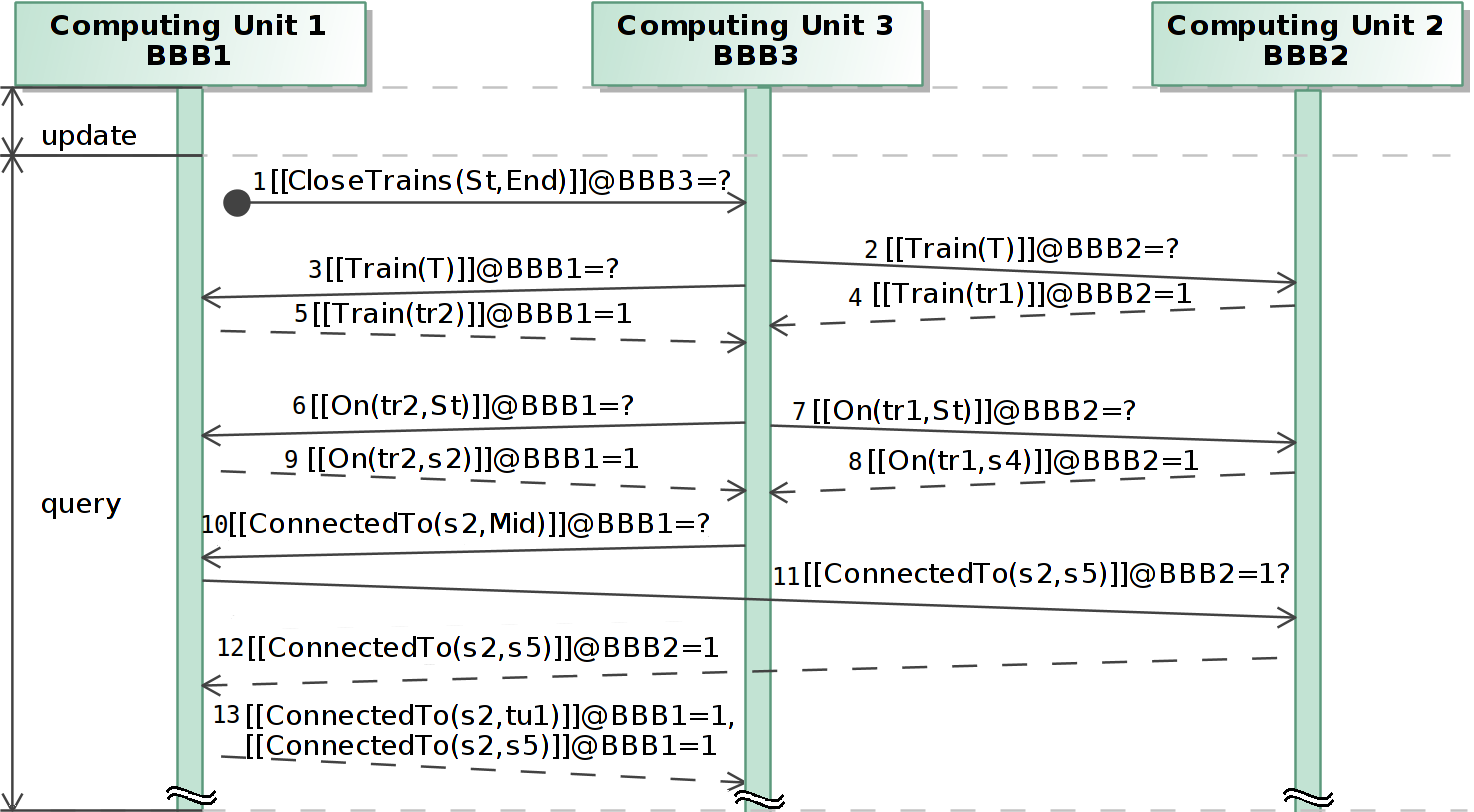
\includegraphics[width=1\textwidth]{figures/seq-diagram-query-exec.png}
	\end{center}
\end{figure}
\todo{ábra okosítás}

